% Add `ngerman` to documentclass for German docs
\documentclass[12pt, a4paper]{article}
\usepackage{a4wide}
\usepackage{setspace}
\usepackage{csquotes}
\usepackage[utf8]{inputenc}

\usepackage{url}
\usepackage[hidelinks]{hyperref}
\usepackage{minted}
\usemintedstyle{perldoc}

% inline code
\newcommand{\code}[1]{\texttt{#1}}

% Uncomment for German
%\usepackage[ngerman]{babel}

% For generating template dummy text
\usepackage{lipsum}

\usepackage{myColors}
\usepackage{myFooter}
\usepackage{myTitle}

% Libraries outside of template
\usepackage[T1]{fontenc}
\usepackage{upquote}
\AtBeginDocument{%
    \def\PYZsq{\textquotesingle}%
}

\usepackage{amsmath}

%%%%%%%%%%%%%%%%%%%%%%%%%%%%%%%%%%%%%%%%%%%%%%%%%%%%%%%%%%%%%%%%%%%%%%%

\project{CS 432 Web Science}
\author{Derek Goddeau}
\title{Assignment Six}
\supervisor{Michael L. Nelson}

\doublespace
\pagestyle{hacker}

\begin{document}
\maketitle

\newpage



%%%%%%%%%%%%
% Facebook %
%%%%%%%%%%%%
\section{Use D3 to visualize Twitter followers}

\subsection{Getting the data}

The data required to create the graph consists of the nodes and the links between them. The desired node data includes username, real name, user ID number and the users profile image. The link data that is needed consists of source nodes and the target nodes they are connected to. The \href{https://github.com/bear/python-twitter}{python-twitter} package is used to obtain the data, first using the \code{api.GetFollowers()} method to get a list of all of the target users followers as \code{User} objects, then creating a Python dictionary to hold the data.


\begin{minipage}{\linewidth} % prevent splitting between pages
\vspace{2em}
\begin{minted}[fontfamily=tt]{python}
data = { 'nodes' : [], 'links' : [] }
for user in users:
    user_data = {   'id': user.id,
                    'name': user.name,
                    'profile_image_url': user.profile_image_url,
                    'screen_name': user.screen_name,
                    'default_profile_image': user.default_profile_image
                }
    data['nodes'].append(dict(user_data))
\end{minted}
\vspace{2em}
\end{minipage}

Then to generate the link data a \code{friends} function to determine if two users follow the other can be wrapped up in a loop over all of the user objects. Because it uses the \code{api.ShowFriendship()} method it is rate limited to 180 calls per 15 minutes. The \code{python-twitter} API is instantiated with \code{sleep\_on\_rate\_limit=True} so that will be the cause if this takes a long time. Use of \code{itertools.combinations()} ensures no wasted calls eat up more time than needed.


\newpage
\noindent
To calculate the time to run on a set of users where $n$ is the number of users:

$$
    \dfrac{\left(\dfrac{\dbinom{n}{2}}{180}\right)\cdot15}{60}\:=\: \text{Time in Hours}
$$

\noindent
Which works out to about 7 hours to generate links between 100 users and just over two weeks for 700 users. Because of this the data collected using the loop below was cut off after 48 hours of runtime which generated over 350 links between over 600 users. For completeness it is still running on a spare server with a uninterruptible power supply, and wrapped up in a catch-all-exceptions loop and the graph will be updated after completion.

\begin{minipage}{\linewidth} % prevent splitting between pages
\vspace{2em}
\begin{minted}[fontfamily=tt]{python}
for alice, bob in combinations(users, 2):
    friendship = friends(alice.screen_name, bob.screen_name)
    if friendship[0]: # alice following bob
        link = { 'source': alice.screen_name,
                 'target': bob.screen_name
               }
        data['links'].append(dict(link))
    if friendship[1]: # alice followed by bob
        link = { 'source': bob.screen_name,
                 'target': alice.screen_name
               }
        data['links'].append(dict(link))
\end{minted}
\vspace{2em}
\end{minipage}


\newpage
\subsection{Graphing the data}

To graph the data I looked everywhere for anything to not write JavaScript or D3 and unfortunately while there are some python wrappers they are either old and have not been updated or they only support a minimal and very restrictive portion of D3. Fortunately \code{NetworkX} is capable of \href{https://networkx.github.io/documentation/networkx-1.10/reference/readwrite.json_graph.html}{dumping a network graph in a D3 ready JSON format}. Since Jupyter Noteboks support the \code{\%\%javascript} magic it was possible to dump the Python data to JSON and then move right on to JavaScript in the next block.

Having never used JavaScript for anything beyond standard website usage and the credit for the code goes to the internet in general and Mike Bostock who wrote the \href{http://mbostock.github.com/d3/ex/force.html}{script that I modified}. The key modification was changing the nodes from circles to the users profile images and resizing on mouseover. This only required adding the \code{"xlink:href"} attribute and \code{.on()} events and then updating the positions properly each tick.

The graph is quite large with even less than half of the dataset, when the full dataset is gathered it may be neccisary to choose some random $x$ number of nodes to graph for perfomance purposes. This method of generating interactive graphs for the web, while nontrivial to learn, seems to have much more potential than other methods like Plotly. To view a live version of the graph click the Jupyter Notebook screenshot below.

\vspace{2em}
\begin{figure}[h]
    \centering
    \href{http://datenstrom.gitlab.io/cs532-s17/d3_twitter_graph/force.html}{
        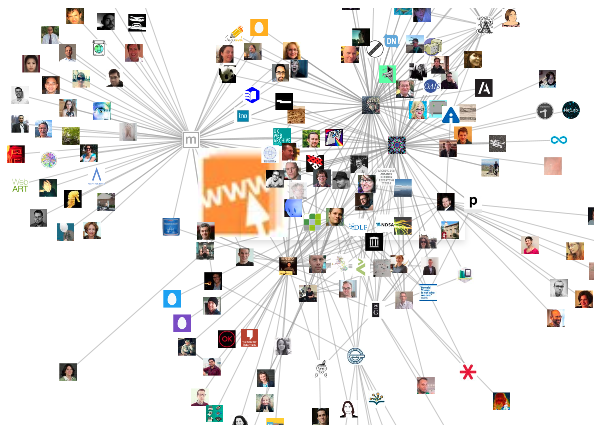
\includegraphics[width=0.50\textwidth]{dia/graph.png}
    }
\end{figure}

\end{document}
